%=====================================================================
\chapter{Installing \tuprolog{}}
\label{installation}
%=====================================================================

Quite obviously, the installation procedure depends on the platform of choice.
For Java, Microsoft .NET and Android, the first step is to manually download the desired distribution (or even just the single binary file) from the \tuprolog{} web site, \texttt{tuprolog.alice.unibo.it}, or directly from the Google code repository, \texttt{tuprolog.googlecode.com}; for Eclipse the procedure is different, since the plug-in installation has to be performed via the Eclipse Plugin Manager.

As a further alternative, users wishing to have a look at \tuprolog{} and trying it without installing anything on their computer can do so by exploiting the `Run via Java Web Start' option, available on the \tuprolog{} web site.

\section{Installation in Java}

The complete Java distribution has the form of a single \texttt{zip} file which contains everything (binaries, sources, documentation, examples, etc.) and unzips into a multi-level directory tree, similar to the following (only first-level sub-dirs are shown):

\begin{Verbatim}[frame=single, framerule=0.5mm, samepage=true, boxwidth=5cm]
    2p
    |---ant
    |---bin
    |---build
    |   |---archives
    |   |---classes
    |   |---release
    |   |---reports
    |   |---tests
    |---doc
    |   |---javadoc
    |---lib
    |---src
    |---test
    |   |---fit
    |   |---unit
    |---tmp
    |---test
\end{Verbatim}

An alternative distribution, without sources, is also available in the \textit{Download} section of the \tuprolog{} repository: obviously, in this case only a subset of the above folders is present (namely, only \texttt{bin}, \texttt{doc}, \texttt{lib} and \texttt{reports}).

If you are only interested in the Java binaries, just look into the \texttt{build/archives} directory, which contains two JAR files:
%
\begin{itemize}
%
\item \texttt{2p.jar}, which contains everything you need to use \tuprolog{},
  such as the core API, the \texttt{Agent} application, libraries, GUI,
  etc.; this is a runnable JAR, that open the \tuprolog{} IDE when double-clicked.
%
\item \texttt{tuprolog.jar}, which contains only the core part of \tuprolog{},
  namely, what you will need to include in a Java application project to be able to access the \tuprolog{} classes, and write multi-paradigm Java/Prolog applications.
\end{itemize}

The other folders contain project-specific files: \texttt{src} contains all the sources, \texttt{doc} all the documentation, \texttt{lib} the libraries used by the \tuprolog{} project, \texttt{test} the sources for the \tuprolog{} test suite (partly as FIT test, partly as JUnit tests), \texttt{ant} some Ant scripts to automate the build of parts of the \tuprolog{} project, etc.


\section{Installation in .NET}

The complete .NET distribution has also the form of a single \texttt{zip} file containing everything; however, due to the automatic generation of \tuprolog{} .NET binaries via IKVM from Java (more on this in Chapter \ref{ch:mpp-in-dotnet}), the unzipped directory tree is simpler, as there are no sources (and therefore no tests, no ant tasks, etc), except for \texttt{OOLibrary} and Conventions, which are NET-specific and therefore written in C\#.
%
So, the resulting tree is similar to the following:
%
\begin{verbatim}
    2p
    |---build
    |   |---examples
    |   |---lib
    |---OOLibrary
    |   |---Conventions
    |   |---Fixtures
    |   |---OOLibrary
\end{verbatim}
%
Here, too, an alternative distribution, without the OOLibrary and conventions sources, is also available in the \textit{Download} section of the \tuprolog{} repository: again, only a subset of the above folders is present in this case.

The .NET binary, \texttt{2p.exe}, can be found in the \texttt{build} folder.


\section{Installation in Android}

The Android distribution has the form of a single \texttt{apk} file, to be installed via install mechanism provided by the Android OS.
So, unless you are interested in the implementation details, there should be no need to download the whole project distribution.
If, however, you like to do so, you will eventually get to a directory tree similar to the following (only the most relevant first-level sub-folders are shown):
%
\begin{verbatim}
    2p
    |---assets
    |---bin
    |   |---classes
    |   |---res
    |---doc
    |---gen
    |---libs
    |---res
    |---screenshots
    |---src
\end{verbatim}
%
The APK binary can be found into the \texttt{bin} folder.

As for the Java case, the other folders contain project-specific files: in particular, \texttt{src} contains the sources, \texttt{res} the Android resources automatically generated during the project build process, \texttt{libs} the libraries used by this project---mainly, the \texttt{tuprolog.jar} file of the corresponding Java version, imported here as an external dependency.


\section{Installation in Eclipse}

The installation procedure is different for the Eclipse platform due to the need to conform to the Eclipse standard procedure for plug-in installation via Plugin Manager.
%Please see the specific section on the \tuprolog{} web site for detailed, screenshot-driven instruction.
%
In order to exploit Eclipse's built-in plugin installation manager, a properly-configured \textit{update site}
must be added to the Eclipse Update Site List first.

To do so:

\begin{enumerate}
  \item open the Eclipse preferences (menu Window $>$ Preferences) and choose the Install/Update item
  and choose the Available Software Sites sub-item. You might want to type ``tuprolog'' in the text field 
  just to check that no other update sites are already defined for it.

  \item now click on the ``Add'' button to add a new software site: in the dialog that appears, type a 
  description in the upper field (e.g. ``tuProlog update site''), and enter the following URL in the lower field:\\
     {\footnotesize{\texttt{http://tuprolog.googlecode.com/svn/2p-plugin/trunk/tuPrologUpdateSite/}}}\\
  The dialog should now look as in Figure \ref{fig:tuPrologPluginInstall-12}.
  Clicking OK, you should now see the new site in the site list.

  \item close this window, and go back to the main Eclipse window. Open the Help menu and choose the 
  \textit{Install new software} item (Figure \ref{fig:tuPrologPluginInstall-34}, top).
  Select the \tuprolog{} software by typing ``tuProlog'' in the filter text field, or by scrolling the site 
  list: after selecting the site, you should see something like the window shown in 
  Figure \ref{fig:tuPrologPluginInstall-4}, bottom.

  \item Now select the \tuprolog{} feature by clicking on the checkbox. If multiple feature versions are 
  proposed (that depends whether you checked the ``show older versions'' option), choose the version you 
  prefer: if unsure, select the most recent.
  Once selected, click Next: installation will take place automatically.
\end{enumerate}

The \tuprolog{} plugin is now installed on your Eclipse system.

\begin{figure}
\centering
  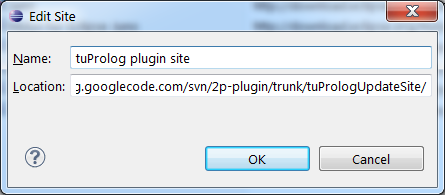
\includegraphics[width=300px]{images/tuPrologPluginInstall-1.png}\\
  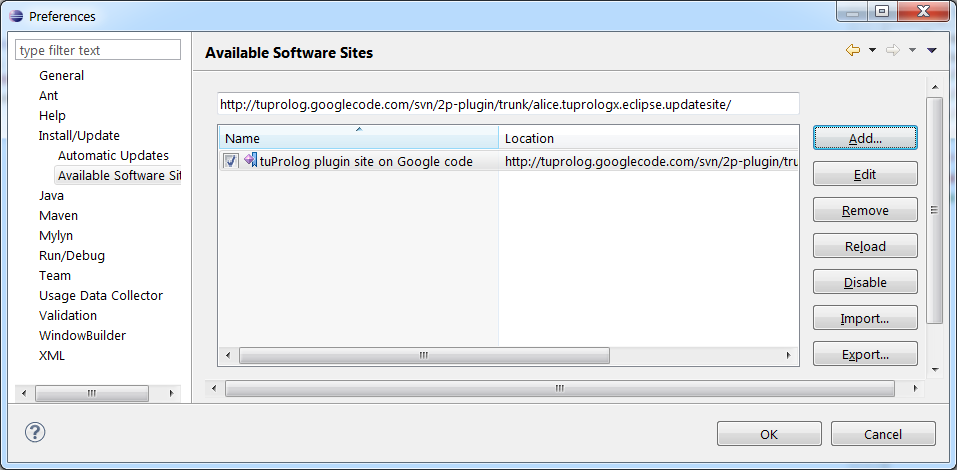
\includegraphics[width=300px]{images/tuPrologPluginInstall-2.png}
  \caption{Plugin installation: adding the Update Site, phase 1}\label{fig:tuPrologPluginInstall-12}
\end{figure}

\begin{figure}
\centering
  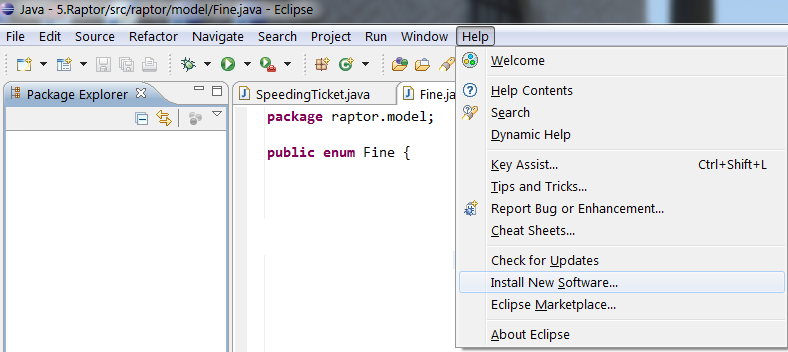
\includegraphics[width=300px]{images/tuPrologPluginInstall-3.png}\\
  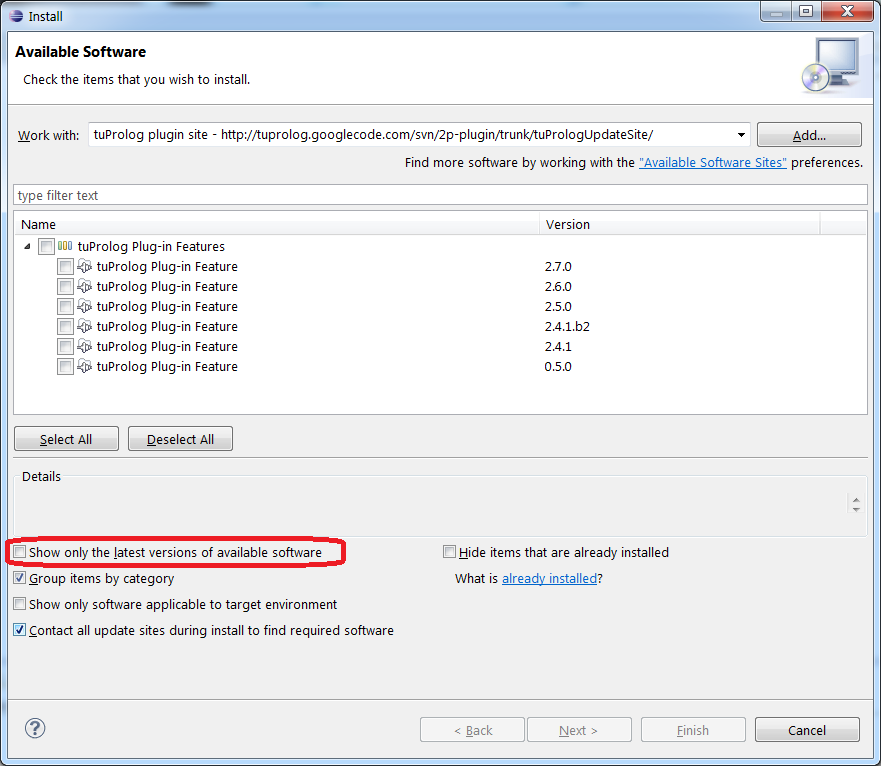
\includegraphics[width=300px]{images/tuPrologPluginInstall-4.png}
  \caption{Plugin installation: adding the Update Site, phase 2}\label{fig:tuPrologPluginInstall-34}
\end{figure}
